\documentclass[a4paper,10pt]{article}
\usepackage[utf8]{inputenc}
\usepackage[MeX]{polski}
\usepackage{graphicx}

\title{[MBI.A] Asembler DNA, sparowane końce - dokumentacja wstępna}
\author{Michał Aniserowicz, Jakub Turek}
\date{}

\begin{document}

\maketitle

\section*{Opis problemu}

Zadanie polega na implementacji aplikacji, która umożliwia tworzenie \emph{scaffoldów} na podstawie dostarczonych zbiorów \emph{contigów} oraz sekwencji PET. 

\begin{center}
  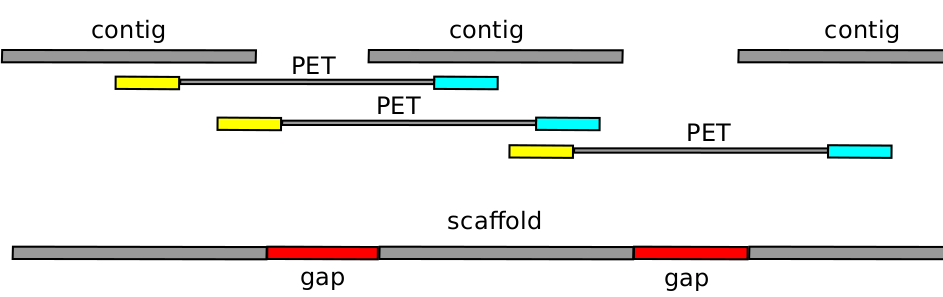
\includegraphics[width=.9\textwidth]{contig_pet.png}
\end{center}

\section*{Założenia}

W~ogólnym przypadku rekonstrukcja sekwencji \emph{contigów} nie jest możliwa. Z~tego względu, na potrzeby projektu przyjęto następujące założenia:

\begin{itemize}
  \item Początki i~końce łańcuchów PET to sekwencje unikalne. Wystąpienie takiej sekwencji w~jednym z~\emph{contigów} oznacza, że jest to odpowiednio początek lub koniec sekwencji PET.
  \item Badane są wyłącznie takie permutacje \emph{contigów}, dla których wystąpienie początku sekwencji PET implikuje przynajmniej częściowe wystąpienie jej końca w~dalszej części łańcucha. Innymi słowy początek lub koniec sekwencji PET nie może w~całości wystąpić w~przerwie (\emph{gap}) \emph{scaffoldu}.
  
    \begin{itemize}
	  \item Wyjątkiem od tej reguły jest początek i~koniec \emph{scaffoldu}, gdzie mogą występować, odpowiednio, niesparowane końce lub początki sekwencji PET.
    \end{itemize}
  
  \item Sekwencje należące do różnych par sparowanych końców mogą częściowo zachodzić na siebie.
\end{itemize}

\section*{Algorytm}

Do rozwiązania zadania użyty zostanie algorytm typu brute-force działający według następującego schematu:

\begin{enumerate}
 \item Wybierana jest początkowa permutacja \emph{contigów}.
 \item Dla danej permutacji obliczany jest ranking \emph{R}:
   \begin{itemize}
    \item Ranking \emph{R} określa, dla danej kombinacji \emph{contigów}, liczbę pokrywających się zasad dla zbioru dopasowań sekwencji PET do łańcucha.
   \end{itemize}
 \item Sprawdzane jest czy wartość \emph{R} jest większa niż dotychczas uzyskana maksymalna wartość rankingu. Jeżeli tak, rozwiązanie zachowywane jest jako najlepsze.
 \item Algorytm jest powtarzany dla każdej unikalnej permutacji \emph{contigów}.
\end{enumerate}

Sekwencja \emph{contigów} dobierana będzie w~sposób losowy. Jako zadanie dodatkowe może zostać przygotowana heurystyczna strategia doboru permutacji.
 
\section*{Implementacja}

Projekt zostanie zaimplementowany w~języku C\#\footnote{W~przypadku, gdy wybór technologii będzie rzutował na obniżenie oceny końcowej (brak przenośności) projekt zostanie zaimplementowany w~języku Java.} (platforma .NET). Testy jednostkowe zostaną napisane w~oparciu o~platformę Visual Studio Unit Testing Framework, z~użyciem bibliotek Moq\footnote{http://code.google.com/p/moq/} oraz AutoMoq\footnote{https://github.com/darrencauthon/AutoMoq}.

Aplikacja będzie posiadała interfejs okienkowy stworzony w~technologii WPF, umożliwiający odczyt danych wejściowych z/zapis danych wyjściowych do pliku. Na dane wejściowe składają się:

\begin{itemize}
 \item Opis \emph{conitgów} w~postaci łańcuchów tekstowych oddzielonych znakami nowej linii.
 
  \begin{verbatim}
    ACAGCTTA
    CCGGGTAC
    TACAGCTT
  \end{verbatim}
  \item Opis sekwencji PET w~postaci dwóch sekwencji (początek, koniec) oraz długości łańcucha. Dane w~sekwencji oddzielone przecinkami, natomiast kolejne PET'y oddzielone znakami nowej linii.
  
  \begin{verbatim}
   GATC,CCAT,100
   GGCT,AGAA,1500
  \end{verbatim}
\end{itemize}

Dane wyjściowe to uporządkowana sekwencja \emph{contigów} oddzielonych znakami spacji reprezentującymi długość przerwy (\emph{gap}).

  \begin{verbatim}
   CCGGGTAC       TACAGCTT  ACAGCTTA
  \end{verbatim}

\section*{Przykład}

\begin{itemize}
 \item Plik wejściowy:
  \begin{verbatim}
   ACAGCTTA
   CCGGGTAC
   TACAGCAA

   CCG,TACA,15
   GCA,GCT,13
  \end{verbatim}
 \item Plik wyjściowy:
  \begin{verbatim}
   CCGGGTAC   TACAGCAA   ACAGCTTA
  \end{verbatim}
\end{itemize}

\end{document}